\documentclass[../main/Feedback.tex]{subfiles}
\begin{document}



\section{Introduction}

\section{Figures/Captions}

\begin{figure*}
  \centering
  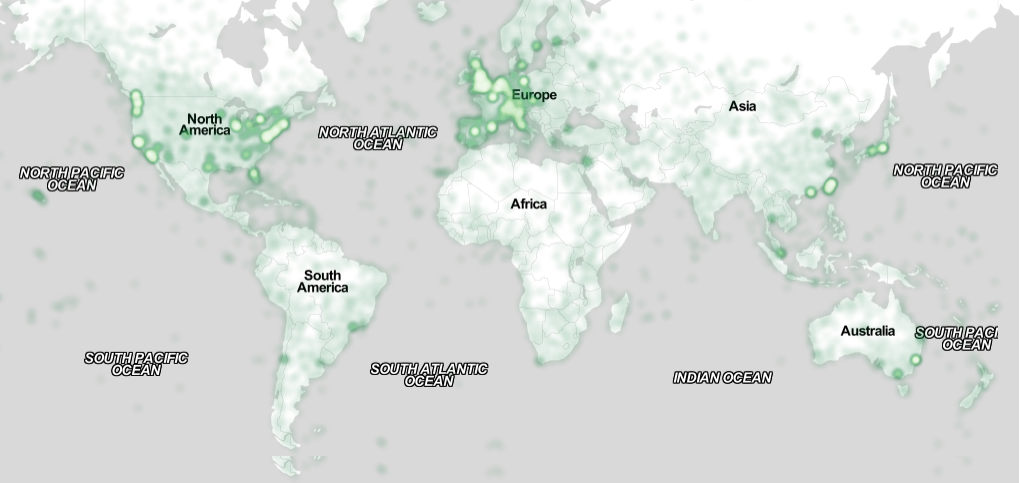
\includegraphics[width=1.75\columnwidth]{../figures/map}
  \caption{In this image, the map maximizes use of space. You can make
    figures as wide as you need, up to a maximum of the full width of
    both columns. Note that \LaTeX\ tends to render large figures on a
    dedicated page. Image: \ccbynd~ayman on
    Flickr.}~\label{fig:figure2}
\end{figure*}

 ``Table~\ref{tab:table1}'' or
``Figure~\ref{fig:figure1}''),

Quotations may be italicized when \textit{``placed inline''}

\begin{quote}
Longer quotes, when placed in their own paragraph, need not be
italicized or in quotation marks when indented (Ramon, 39M).
\end{quote}

\section{Language, Style, and Content}

The written and spoken language of SIGCHI is English. Spelling and
punctuation may use any dialect of English (e.g., British, Canadian,
US, etc.) provided this is done consis- tently. Hyphenation is
optional. To ensure suitability for an international audience, please
pay attention to the following:

\section{Conclusion}




% just remove comment on last page for ballancing columns.
%\balance{}

\end{document} 